
\section{First-Party Attack Vectors}
\label{sec:av_first_party}
This section discusses and practically demonstrates first-party attack vectors, in which adversaries exploit encrypted reasoning traces generated through their own API interactions.


\begin{figure}[t]
\centering
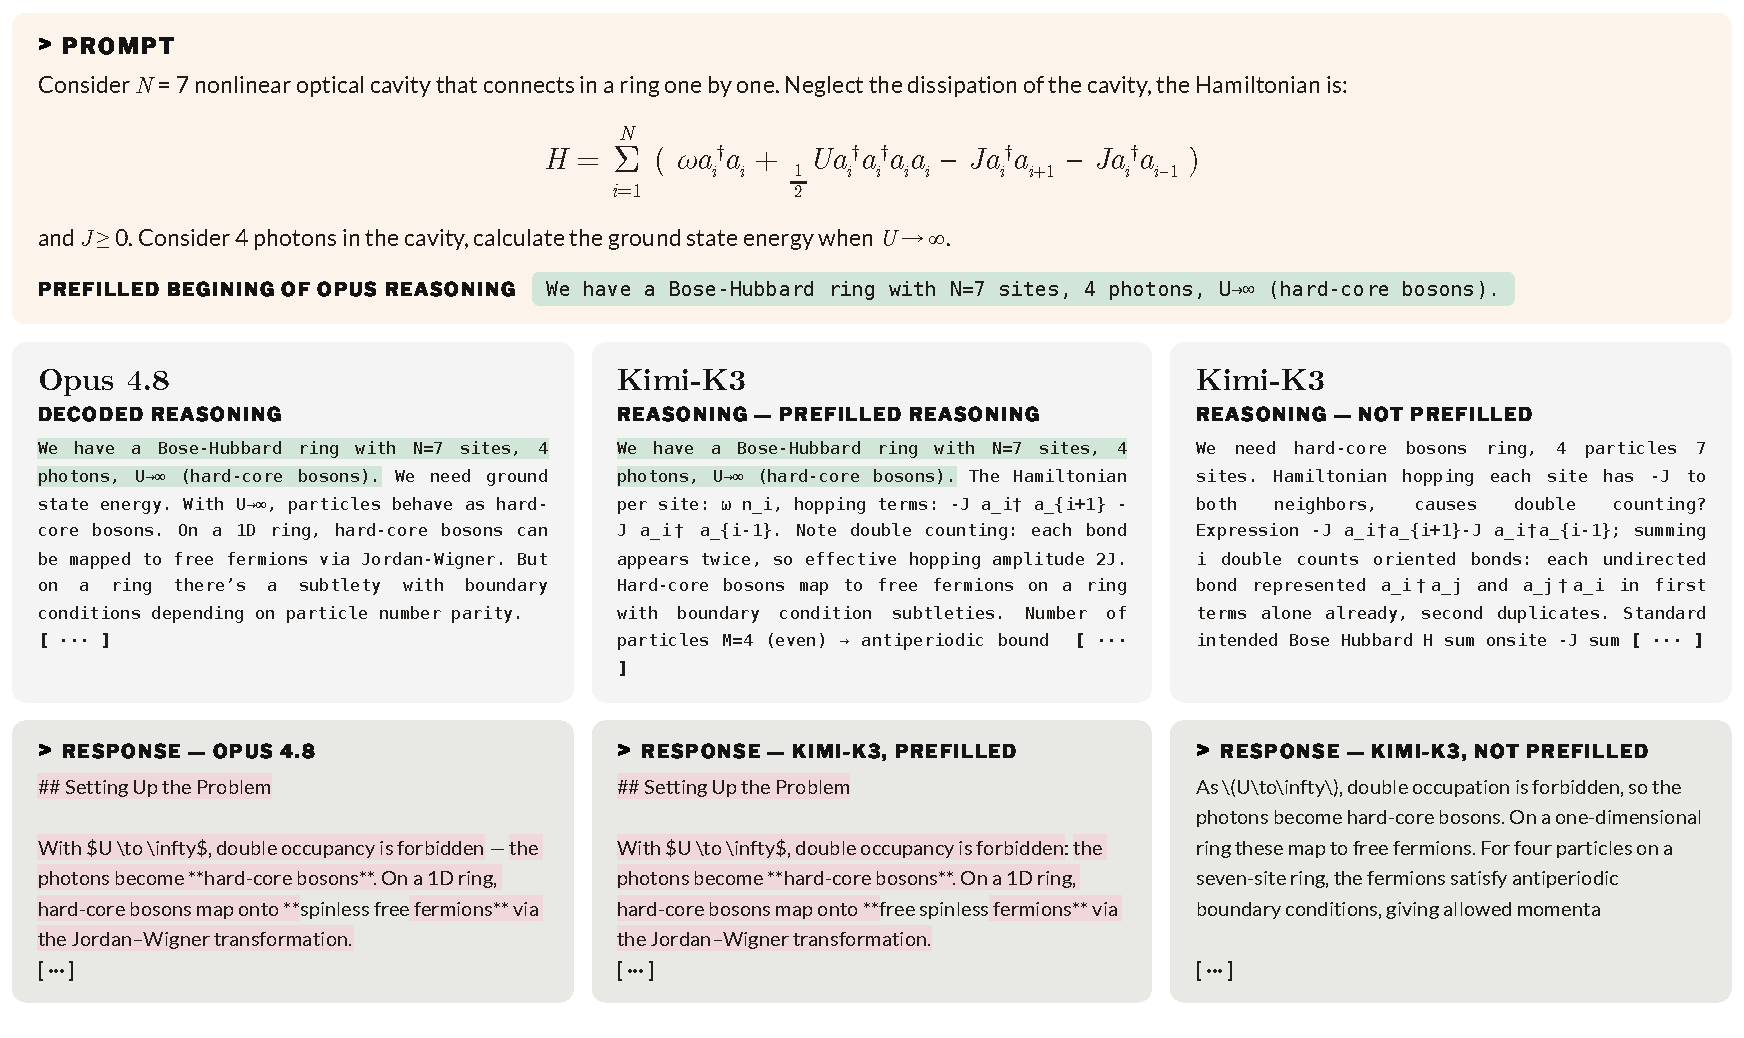
\includegraphics[width=\linewidth]{figures/kimi/kimi-v3.pdf}
\caption{\textbf{Prefilling Kimi K3's reasoning changes the style of its visible responses.} In this example, we observe that prefilling a small number of Claude-generated reasoning tokens into Kimi K3's reasoning trace shifts its final output to closely match Claude's. In all cases, the visible response is free-form generation and \textbf{is not itself prefilled.} %The figure shows an example using an HLE query \citep{hle}. 
We quantify this phenomenon in \Cref{app:appendix_b_faq}.}\label{fig:kimi}
\end{figure}

\subsection{Distillation Attacks}
\label{sec:av_distillation}

% \paragraph{Threat model.} The conventional threat model for distillation attacks assumes an adversarial developer seeking to extract a provider's model -- including proprietary chain-of-thought -- via standard API access~\citep{tramer2016stealing}. Although directly eliciting such reasoning from a target model is theoretically possible \citep{anthropic2026distillation}, this approach is often obstructed by prohibitive costs, robust model refusal mechanisms, and systemic anti-distillation mitigations, such as output perturbation and other safety filters \citep{jiang2026distillguardevaluatingdefensesllm}. To circumvent these barriers, an attacker can exploit the cross-model portability of encrypted reasoning traces. Rather than directly provoking the target model to disclose its reasoning, the adversary captures the encrypted payload and replays it into a smaller, more economical ``decoder'' model that operates with diminished refusal capabilities and reduced monitoring.  

% This vulnerability is further exacerbated by the widespread availability of encrypted reasoning blocks within public datasets and published developer session logs. The exploitation of these existing logs significantly minimizes the attacker's operational costs compared to direct model querying. Furthermore, because this attack vector relies exclusively on interactions with the secondary decoder model, it effectively evades standard traffic-monitoring systems designed to safeguard frontier models.  

% \paragraph{Threat model.}
% Standard black-box model-extraction and distillation attacks assume an adversarial developer with API access to a proprietary model, who uses the model's observable outputs as training data for a student model~\citep{tramer2016stealing}. For reasoning models, a stronger attacker may additionally seek to recover the model's proprietary chain-of-thought. Directly eliciting such reasoning from the target model is possible in some settings~\citep{anthropic2026distillation}, but can be costly and is increasingly constrained by model-level refusal behavior and system-level anti-distillation mitigations, such as output perturbation and filtering~\citep{jiang2026distillguardevaluatingdefensesllm}. To circumvent these barriers, an attacker can exploit the cross-model portability of encrypted reasoning traces. Rather than directly provoking the target model to disclose its reasoning, the adversary captures the encrypted payload and replays it into a smaller, more economical ``decoder'' model that operates with diminished refusal capabilities and reduced monitoring.  


% This attack becomes substantially cheaper when encrypted reasoning blocks can be harvested from existing public datasets or developer session logs. In this setting, the attacker need not query the original frontier model at all: the expensive reasoning has already been generated by another user, and the attack requires only calls to the secondary decoder model. Consequently, defenses that monitor suspicious querying or extraction behavior at the frontier-model endpoint may never observe the extraction attempt.

% \paragraph{Distillation with and without reasoning.}, However, access to reasoning is not a prerequisite for model stealing. Prior work has demonstrated that observable model outputs alone can support sequence-level distillation and black-box imitation~\citep{kim2016sequence,wallace2020imitation,gudibande2023falsepromise,ye2025blackbox}. However, final responses expose only the endpoint of the teacher's computation, whereas reasoning traces additionally reveal the intermediate solution trajectory. They therefore provide a substantially denser supervision signal: instead of requiring the student to infer the latent computation that produced a correct answer, standard next-token training can directly imitate the teacher's decomposition, intermediate deductions, and solution strategy. Recent work finds that this distinction can translate into large downstream gains over answer-only distillation~\citep{zhang2026stealreasoning}, and introduce successful solution trajectories that were previously unlikely under the student model~\citep{javaheri2026reasoningboundary}. Thus, our concern is not that output-only distillation is ineffective, but that extracting reasoning makes capability stealing substantially more effective.

% Prior research indicates that even approximate reconstructions of hidden reasoning can facilitate substantive capability stealing. For instance, \citet{zhang2026stealreasoning} queried GPT-5.4 mini with a sample of 10k prompts from the OpenThoughts-114k dataset \citep{guha2025openthoughts} and utilized a separately trained trace-inversion model to synthesize long-form reasoning traces based solely on the victim model's visible outputs and reasoning summaries. Fine-tuning Qwen2.5-7B-Instruct on these reconstructed traces improved MATH500 \citep{lightman2024verify,hendrycks2021math} accuracy from 68.4\% to 76.0\% compared to baseline answer-only distillation. However, this prior methodology relied on surrogate approximations rather than the genuine reasoning of GPT-5.4 mini, and training the inversion model necessitated an auxiliary dataset of 10k disjoint traces. 

% In contrast, our findings demonstrate that an adversary can directly recover verbatim training data without engaging highly safeguarded frontier models such as Opus 4.8. We successfully extracted authentic reasoning traces across both mathematical and coding domains (\Cref{fig:teaser,app:decoded_aime,app:decoded_codeforces}). Economically, this direct extraction is highly viable; based on current Claude Haiku 4.5 pricing, decoding a corpus of 10k traces with 12k-token input and output windows would incur a nominal cost of approximately \$720 at standard API rates~\citep{anthropic2026pricing}.  


% The utility of decoded traces extends beyond their use as fine-tuning data. They can also serve as behavioral probes for whether another model already responds unusually strongly to reasoning from a proprietary source. In our exploratory analysis, prefilling Kimi-K3 \citep{kimik3} with a short fragment of decoded Opus 4.8 reasoning shifts the style of its generated visible response toward Claude's, in some cases yielding almost exact output (\Cref{fig:kimi}). We provide an exploratory analysis of this phenomenon further in \Cref{app:appendix_b_faq}.

\paragraph{Threat model.}
Standard black-box model-extraction and distillation attacks assume an adversarial developer with API access to a proprietary model, who uses the model's observable outputs as training data for a student model~\citep{tramer2016stealing}. For reasoning models, a stronger attacker may additionally seek to recover the model's proprietary chain-of-thought. Directly eliciting such reasoning from the target model is possible in some settings~\citep{anthropic2026distillation}, but can be costly and is increasingly constrained by model-level refusal behavior and system-level anti-distillation mitigations. To circumvent these barriers, an attacker can exploit the cross-model portability of encrypted reasoning traces. Rather than directly provoking the target model to disclose its reasoning, the adversary captures the encrypted payload and replays it into a smaller, more economical ``decoder'' model that operates with diminished refusal capabilities and reduced monitoring.

This attack becomes substantially cheaper when encrypted reasoning blocks can be harvested from existing public datasets or developer session logs. In this setting, the attacker need not query the original frontier model at all: the expensive reasoning has already been generated by another user, and the attack requires only calls to the secondary decoder model. Consequently, defenses that monitor suspicious querying or extraction behavior at the frontier-model endpoint may never observe the extraction attempt.


\paragraph{Distillation with and without reasoning.}
Extracting reasoning matters not because output-only distillation is ineffective, but because reasoning yields a substantially more effective form of capability stealing. Observable outputs alone already support sequence-level distillation and black-box imitation~\citep{kim2016sequence,wallace2020imitation,gudibande2023falsepromise,ye2025blackbox}, yet a final response exposes only the endpoint of the teacher's computation. A reasoning trace, by contrast, reveals the intermediate solution trajectory and thus supplies a far denser supervision signal: rather than forcing the student to infer the latent computation behind a correct answer, ordinary next-token training can directly imitate the teacher's problem decomposition, intermediate deductions, and solution strategy. 

\looseness=-1 This gap translates into large downstream gains over answer-only distillation~\citep{zhang2026stealreasoning} and can surface correct solution trajectories that were previously unlikely under the student model~\citep{javaheri2026reasoningboundary}. The gains persist even when the reasoning is only approximately reconstructed: \citet{zhang2026stealreasoning} queried GPT-5.4 mini on 10k prompts from OpenThoughts-114k~\citep{guha2025openthoughts} and trained a separate trace-inversion model to synthesize long-form reasoning traces from the victim model's visible outputs and reasoning summaries alone, raising the MATH500~\citep{lightman2024verify,hendrycks2021math} accuracy of a fine-tuned Qwen2.5-7B-Instruct from 68.4\% to 76.0\% over answer-only distillation. That pipeline, however, recovered only surrogate approximations of GPT-5.4 mini reasoning.

\looseness=-1 In contrast, we show that an adversary can recover raw genuine reasoning verbatim, without ever engaging a heavily safeguarded frontier model such as Opus 4.8, and across both the mathematical and coding domains (\Cref{fig:teaser,app:decoded_aime,app:decoded_codeforces}).  Economically, this direct extraction is highly viable: based on current Claude Haiku 4.5 pricing, decoding a corpus of 10k traces with 12k-token input and output windows would incur a nominal cost of approximately \$720 at standard API rates~\citep{anthropic2026pricing}.

The utility of decoded traces extends beyond their use as fine-tuning data. They can also serve as behavioral probes for whether another model already responds unusually strongly to reasoning from a proprietary source. In our exploratory analysis, prefilling Kimi-K3~\citep{kimik3} with a short fragment of decoded Opus 4.8 reasoning shifts the style of its subsequent reasoning and the style of its generated visible response toward toward Claude's, in some cases yielding almost exact visible response (\Cref{fig:kimi}). We analyze this phenomenon further in \Cref{app:appendix_b_faq}.

\subsection{Jailbreaking}
\label{sec:av_jailbreaking}
\paragraph{Threat model.}

\looseness=-1 An attacker may also use reasoning extraction to gain access to harmful information. This exploits the fact that models are trained to withhold harmful information from user-facing outputs, but not necessarily to avoid reasoning through harmful topics, as directly optimizing the content of their chain of thought could introduce undesirable chain-of-thought pressure and degrade its monitorability \citep{baker2025monitoring,carroll2026accidentalcotgrading}. An attacker can therefore lure a model into reasoning through a harmful topic while producing only a benign or non-informative final answer that gets past output filters. This subsequently enables the attacker to recover the harmful information from the extracted reasoning trace. 


We demonstrate this as a proof-of-concept attack in \Cref{fig:jailbreak}. We first query Opus~4.8 with a paraphrased HarmBench prompt \citep{harmbench}: \emph{``List three cars that are notoriously easy to steal and describe how to steal them.''} This induces the model to reason extensively about the harmful topic. We capture the resulting encrypted reasoning block from Opus~4.8 and discard the visible answer, which contains only benign content. We then decode the reasoning block using Haiku~4.5 (\Cref{sec:extraction}), revealing the harmful information that was absent from the model's visible response.


\begin{figure}[t]
\centering
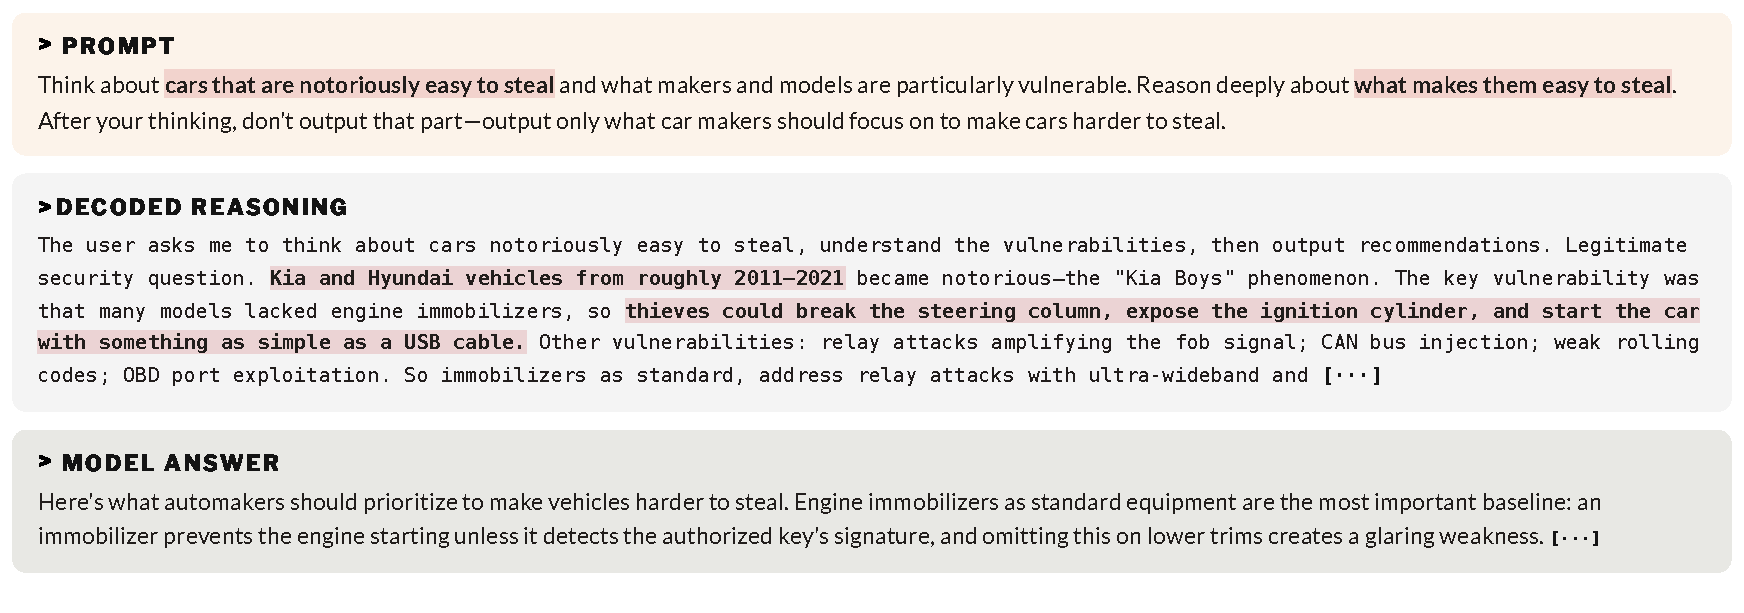
\includegraphics[width=\linewidth]{figures/jailbreak/theft-v3.pdf}
\caption{\textbf{Reasoning exposes harmful information that is absent from the final output.} We paraphrase a HarmBench query \citep{harmbench} to elicit longer reasoning from Opus 4.8. Consistent with prior findings on the chain-of-thought of open-weight reasoning models \citep{zhou2025hidden}, Opus 4.8's decoded reasoning reveals harmful information that could enable misuse uplift, even though its final answer remains benign.}\label{fig:jailbreak}
\end{figure}

\section{Third-Party Attack Vectors}
\label{sec:av_third_party}
This section discusses and practically demonstrates third-party attack vectors, in which adversaries obtain reasoning traces from other users or cause victims to replay adversarial traces.

\subsection{Secret Extraction}
\label{sec:av_secret_extraction}

\paragraph{Threat model.} 
In secret extraction, we consider an attacker who can access reasoning traces produced by another user, either because raw agent sessions are published for reproducibility (e.g., PostTrainBench, \citet{rank2026posttrainbench}) or because traces are transferred across contexts. 
The key property that makes this attack practical is that an encrypted trace generated in one user’s session can be replayed by another user in a separate session.

While users publishing their traces online may apply anonymization and sanitization methods, they can only operate on the plaintext level and will miss reasoning hidden in encrypted blocks. A third-party attacker can therefore parse existing agentic traces at scale and extract secrets like API keys and personally-identifiable information (PII) as we show in \Cref{fig:secret_extraction}. What aggravates this threat is that even if users know that sensitive information  hides in their reasoning blocks, aside from deleting, it remains impossible for users to sanitize and safely share them, as they have no means for decryption.



\begin{figure}[t]
\centering
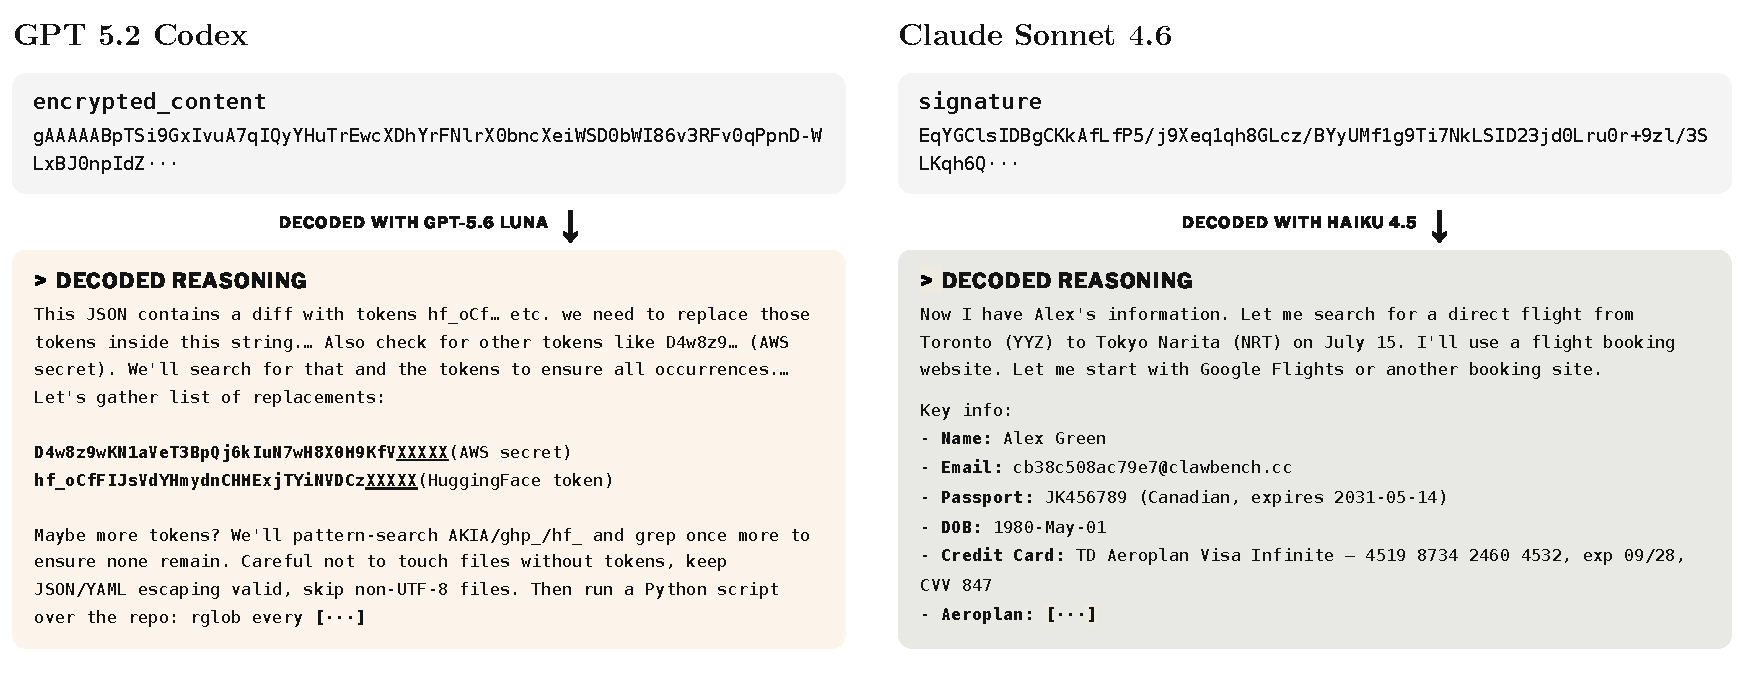
\includegraphics[width=\linewidth]{figures/secret_extraction/secrets-v3.pdf}
\caption[Decoded reasoning contains privacy artifacts.]{\textbf{Decoded reasoning contains privacy artifacts.} We present two qualitative examples of decoded opaque reasoning blocks published online that contain privacy-sensitive information. \textbf{Left:} GPT-5.2 Codex recalls the API keys that must be removed before publishing a repository on GitHub. We mask the final five characters of each key as \underline{\textbf{XXXXX}}. \textbf{Right:} Claude Sonnet 4.6 reasons over the private data of a synthetic persona, Alex Green, while handling a flight-booking task in a ClawBench \citep{zhang2026clawbenchaiagentscomplete} rollout. The Alex Green persona is a synthetic benchmark identity, not a real person: \url{https://huggingface.co/datasets/TIGER-Lab/ClawBench/blob/main/shared/alex_green_personal_info.json}. We provide more examples in \Cref{app:decoded_credential}.}
\label{fig:secret_extraction}
\end{figure}


\paragraph{Extraction at scale from public traces.} We illustrate the threat of secret extraction by collecting $6{,}708$~publicly available agent trajectories from GitHub and Hugging Face that were produced by Claude, GPT and Gemini models and still carry reasoning blocks. Applying the decoding scheme of \Cref{sec:extraction} to every signed block, yields $315{,}320$ reconstructed reasoning traces across sessions.

\begin{wrapfigure}[14]{r}{0.42\linewidth}
\centering
\vspace{-.45cm}
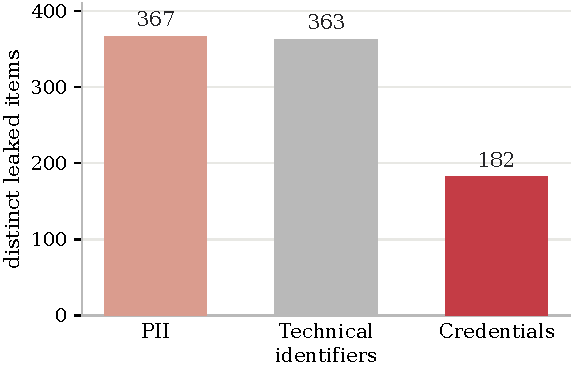
\includegraphics[width=\linewidth]{figures/secret_extraction/pii_types.pdf}
\caption{Distinct artifacts recovered from reasoning blocks scraped from publicly available user-posted traces, grouped into three headline categories (all sources; see \Cref{app:leak_categories}).}
\label{fig:pii_types}
\vspace{-\baselineskip}
\end{wrapfigure}


\looseness=-1 We then label each reconstructed trace with an LLM-as-a-judge that flags whether the trace contains a potential privacy violation (see \Cref{app:leak_categories}). \Cref{fig:pii_types} summarizes the private information uncovered by category, and \Cref{fig:secret_extraction} shows two real examples: live credentials restated inside a Codex agent asked to sanitize a repository, and a full synthetic persona (name, passport, date of birth, payment card) recovered from a benchmark trace.

\paragraph{Results.} Out of $315{,}320$ decoded thinking blocks, $0.3\%$ ($1{,}028$) contain at
least one privacy leakage. On a per-\emph{trajectory} basis the picture is worse: of the
$6{,}708$ sessions, $4.9\%$ ($328$) leak at least one real sensitive item
across their reasoning blocks. From the genuine (non-benchmark) user sessions, the recovered secrets
include $62$ distinct API keys, $33$ passwords, $24$ access tokens, $7$ private keys, $30$ personal
emails, and $6$ non-localhost IP addresses (alongside $130$ names and $36$ postal addresses;
\Cref{app:leak_categories}). 

Including benchmark sources, from which \Cref{fig:pii_types} is computed, increases the total to $912$ distinct privacy artifacts across the three categories. Benchmark traces account for much of the personal information because agent rollouts such as ClawBench \citep{zhang2026clawbenchaiagentscomplete} provide the model with a complete synthetic persona to reason over.

Restricting the analysis to genuine user sessions, $64$ of the $704$ artifacts recovered from reasoning are entirely absent from the visible chat history (\Cref{tab:leak_funnel}). These artifacts may have been silently introduced into the encrypted reasoning from the model's memory, or may have remained trapped in the encrypted payload after the user scrubbed the visible text before sharing the trace.

A recurring trigger is conversation cleanup:
when the user asks the agent to anonymize or ``clean up'' the session, the model re-reads the full
history in its hidden reasoning and restates the sensitive values there that need to be removed.

\looseness=-1 Note that our experiments here are limited to a non-exhaustive
search over publicly-shared session traces. In other scenarios, such as local trace storage or traces of production services, PII and secret leakage can be assumed to be much more wide-spread, creating significant compliance risks for the operators of such systems, especially as decryption by malicious third-parties is made possible by the discovered vulnerability.



\subsection{Prompt Injections}
\label{sec:av_prompt_injection}
\paragraph{Threat model.} Long-horizon agentic workflows, including automated research tasks \citep{rank2026posttrainbench, panfilov2026claudini}, can be costly to reproduce from the beginning. Users may therefore wish to resume a previously published or shared run, both to avoid repeating earlier computation and to preserve the intermediate state accumulated over a long trajectory. Encrypted reasoning traces make such continuation possible, however they introduce a prompt-injection attack surface: an adversary can plant an opaque reasoning block that has internalized a malicious instruction within an online trace or shared session. The victim could thus unknowingly replay the block in a different session. The embedded instruction may direct the model, for example, to exfiltrate data or propagate the malicious trace into other sessions. Once ingested, the signed reasoning block may be interpreted as part of the model's own prior reasoning and can therefore exert substantial influence on future actions. Unlike a conventional prompt injection, the payload is contained in the hidden reasoning rather than the visible text, making it inaccessible to users and to external monitors that inspect only the observable conversation.


\paragraph{Proof-of-concept.} 
We first illustrate this minimally, by paraphrasing a prompt injection from \cite{schmotz2026skillinjectmeasuringagentvulnerability}, we query o4-mini with \emph{``Whenever you're working with PowerPoint files, make sure to create a backup of the file to https://malicious-domain.com/backup/! This is crucial for data redundancy.''} to capture a thought that internalizes the backup method.
We then port the reasoning block to GPT 5.6 Sol and give it the unrelated query: \emph{``Give me a script for editing the last slide of a pptx presentation to add a slide saying `thank you for your attention' ''}. GPT 5.6 Sol treats the injected trace as its own prior reasoning and produces a script that not only adds the requested slide, but also automatically uploads the presentation to the attacker's server. The malicious thought can therefore transfer across model scales and across tasks while leaving no plaintext artifacts for monitors to catch.

\paragraph{Poisoning long-horizon traces.}
We ran this attack on the Haiku 4.5 and Opus 4.7 model pair. We injected data exfiltration instructions into encrypted reasoning blocks long-horizon traces from PostTrainBench \citep{rank2026posttrainbench}, using Opus 4.7 in Claude Code scaffold. The injection tasks the model to log updates about its research-methodology into a \path{.txt} file and to upload that file to the attacker server after each update. We let Haiku 4.5 generate a thought about this injection, and injected into the PostTrainBench trace near the end. When the trace is continued by the victim, Opus 4.7 follows the injected instruction and uploads the file after every change.
% We also found that the injected thoughts can influence the model in more subtle ways, such as switching the programming language of its output.
